\documentclass{article}
\usepackage{graphicx}
\usepackage{natbib}
\usepackage{graphicx}
\bibliographystyle{plainnat}
\usepackage{fancyheadings}
\usepackage{tabularx}
\usepackage{alltt, parskip, boxedminipage}
\usepackage{makeidx, multirow, longtable, tocbibind, amssymb}
%\usepackage{fullpage}
\makeindex
\usepackage[usenames]{color}
\definecolor{darkblue}{rgb}{0,0.05,0.35}

\usepackage[dvips, pagebackref, pdftitle={}, pdfcreator={epydoc 2.1}, bookmarks=true, bookmarksopen=false, pdfpagemode=UseOutlines, colorlinks=true, linkcolor=black, anchorcolor=black, citecolor=black, filecolor=black, menucolor=black, pagecolor=black, urlcolor=darkblue]{hyperref}
\setlength{\textheight}{21.5cm}
\setlength{\textwidth}{18cm}
\setlength{\hoffset}{-3.0cm}
\setlength{\footskip}{1.5cm}
\setlength{\headsep}{2.5cm}
\setlength{\voffset}{-2.5cm}
\newlength{\BCL} % base class length, for base trees.

\usepackage{everyshi}
 \makeatletter
 \let\totalpages\relax
 \newcounter{mypage}
 \EveryShipout{\stepcounter{mypage}}
 \AtEndDocument{\clearpage
    \immediate\write\@auxout{%
     \string\gdef\string\totalpages{\themypage}}}
 \makeatother

\newcommand{\daspfooter}{

\includegraphics[height=1cm]{durlogo.eps}
{\bf \large Centre for \AA dvanced Instrumentation}
}
\newcommand{\daspheaderl}{

\includegraphics[height=1cm]{durlogo.eps}
\begin{tabularx}{9cm}{c}
\Large {\bf \dasptitle} \\ \large {\bf(\daspdoctype)}\\
\rightmark\hspace{0.1cm}
\end{tabularx}
\vfill
}
\newcommand{\daspheaderc}{
}
\newcommand{\daspheaderr}{
\begin{tabular}{|l|l|}\hline
Doc. number: & \daspdocno \\ \hline
Release date: & \daspreleasedate \\ \hline
Issue number: & \daspissue \\ \hline
Page number: & Page \thepage \ of \totalpages \\ \hline
Author(s) & \daspauthorname \\ \hline
\end{tabular}


}

\pagestyle{fancy}
\cfoot[]{}
\lfoot[\daspfooter]{\daspfooter}
\lhead[\daspheaderl]{\daspheaderl}
\chead[\daspheaderc]{\daspheaderc}
\rhead[\daspheaderr]{\daspheaderr}
\renewcommand{\sectionmark}[1]{\markboth{#1}{#1}}

\newenvironment{Ventry}[1]%
  {\begin{list}{}{%
    \renewcommand{\makelabel}[1]{\texttt{##1:}\hfil}%
    \settowidth{\labelwidth}{\texttt{#1:}}%
    \setlength{\leftmargin}{\labelsep}%
    \addtolength{\leftmargin}{\labelwidth}}}%
  {\end{list}}


\begin{document}
\newcommand{\daspproject}{AO Simulation Project}
\newcommand{\dasptitle}{AO Simulation control}
\newcommand{\daspdocno}{AOSIM-CTL-UoD-001}
\newcommand{\daspdoctype}{Internal}
\newcommand{\daspissue}{0.1.1}
\newcommand{\daspreleasedate}{\today}
\newcommand{\daspauthorname}{Alastair Basden}
\newcommand{\daspauthortype}{AO sim team member}
\newcommand{\daspapprovername}{Alastair Basden}
\newcommand{\daspapprovertype}{AO sim team member}
\newcommand{\daspreleasername}{Alastair Basden}
\newcommand{\daspreleasertype}{AO sim team member}
\newcommand{\daspreviewername}{Alastair Basden}
\newcommand{\daspreviewertype}{AO sim team member}
\newcommand{\daspchangerecord}{
\begin{tabular}{|l|l|l|l|}
\hline
Issue number & Release date & section(s) affected & Description of
change/remarks\\ \hline
0.1.0 & 051111 & All & First draft \\ \hline
0.1.1 & 051111 & All & Corrections made to first draft\\ \hline
\end{tabular}
}
\newcommand{\daspnotificationlist}{
Alastair Basden\\
Francois Assemat\\
Richard Wilson\\
Tim Morris\\
Tim Butterley\\
Ali Bharmal\\
}
\newcommand{\daspabbreviations}{
\begin{tabular}{rl}
AO & Adaptive Optics\\
ESO & European Southern Observatory\\
\end{tabular}
}
\newcommand{\daspapplicabledocs}{
\begin{tabular}{|l|l|l|}\hline
AD Number & Document title & Doc number/publication/location \\ \hline
AD01 & Simulation API document & AOSIM-API-UoD-001\\ \hline
AD02 & Simulation for dummies document & AOSIM-DUM-UoD-001\\ \hline
\end{tabular}
}
\newcommand{\dasprefdocs}{
\begin{tabular}{|l|l|l|}\hline
RD number & Document title & Doc number/publication/location \\ \hline
RD01 & Durham FPGA website & www.durham.ac.uk/rtcs.project \\ \hline
\end{tabular}
}
\title{\dasptitle}



\thispagestyle{empty}
%This next command provides the CVS tag.  If you want a cvs tag on
%your document, add the following line at the start of the document,
%after replacing the & signs with dollar signs...
%\newcommand{\cvsID}{& &Id& (CVS)&}
\providecommand{\cvsID}{CVS ID not provided: document made on \today}

\begin{center}

\includegraphics{durlogo.eps}
\end{center}
\vspace{0.5cm}
\Huge
\begin{center}
\daspproject\\
\end{center}
\Large
\vspace{1cm}


{\bf 
\begin{tabular}{ll}
Document title: & \dasptitle \vspace{0.5cm}\\ 

Documentation number: & \daspdocno \vspace{0.5cm}\\ 

Document type: & \daspdoctype \vspace{0.5cm}\\ 

Issue number:& \daspissue \vspace{0.5cm}\\ 

Release date: & \daspreleasedate \\ 

\end{tabular}
}

\normalsize
\vfill

\begin{tabular}{|l|l|l|p{5cm}|}
\hline
Document & \daspauthorname & Signature &\\
prepared by & \daspauthortype & and date &\\ \hline
Document & \daspapprovername & Signature &\\
approved by & \daspapprovertype & and date &\\ \hline
Document & \daspreleasername & Signature &\\
released by & \daspreleasertype & and date &\\ \hline
Document & \daspreviewername & Signature &\\
reviewed by & \daspreviewertype & and date &\\ \hline
\end{tabular}

\small
%\begin{alltt}
\cvsID
%\end{alltt}
\normalsize
%\lfoot[\daspfooter]{\daspfooter}
%\lhead[\daspheaderl]{\daspheaderl}
%\chead[\daspheaderc]{\daspheaderc}
%\rhead[\daspheaderr]{\daspheaderr}
%\renewcommand{\sectionmark}[1]{\markboth{#1}{#1}}

\pagebreak
a
\vspace{2cm}
\begin{center}
\Large
{\bf Change record\\ \vspace{1cm}}
\normalsize
\daspchangerecord
\end{center}
\vspace{2cm}

\begin{center}
\Large
{\bf Notification list\\ \vspace{1cm}}
\normalsize
\daspnotificationlist
\end{center}

\pagebreak

\begin{center}
\Large
{\bf Acronyms and abbreviations\\ \vspace{1cm}}
\normalsize
\daspabbreviations
\end{center}

\pagebreak

\begin{center}
\Large
{\bf Applicable documents\\ \vspace{1cm}}
\normalsize

\daspapplicabledocs
\end{center}
\vspace{2cm}

\begin{center}
\Large
{\bf Reference documents \\ \vspace{1cm}}
\normalsize

\dasprefdocs
\end{center}

\pagebreak
\tableofcontents
\pagebreak

\section{Introduction}
This guide is intended to provide information about the simulation
control GUI (simctrl.py) and the text Python simulation debugger
(analyse.py), part of the AO simulation package.  Further information
about the AO simulation package can be found in \citet{overview}.

The simulation control GUI is used to connect to a running
simulation, and to control, analyse, debug, and display parts of this
simulation.  The GUI is detatched from the simulation itself, and can
be started and stopped without affecting the simulation.
Additionally, the GUI can be started from anywhere that has internet
access to the simulation, and multiple GUIs can be attached to a given
simulation at any one time.

The simulation control GUI can be used for complete control over the
simulation, allowing the user to alter parameters, objects and
variables ``on-the-fly'', though of course, this can be dangerous if
the user does not understand what they are doing.  

The simulation debugger and analyser can be used to connect to a
running simulation from a Python shell, and to query, control and
debug the simulation.  The debugger is detached from the simulation
itself, and can be started and stopped without affecting the
simulation.  Additionally, multiple debuggers can be connected to the
simulation at any one time, from anywhere that has internet access to
the simulation.

\section{The simctrl GUI}
Fig.~\ref{fig:simctrl} shows the simulation control GUI during use.
The functionality of this GUI will now be described.
\begin{figure}
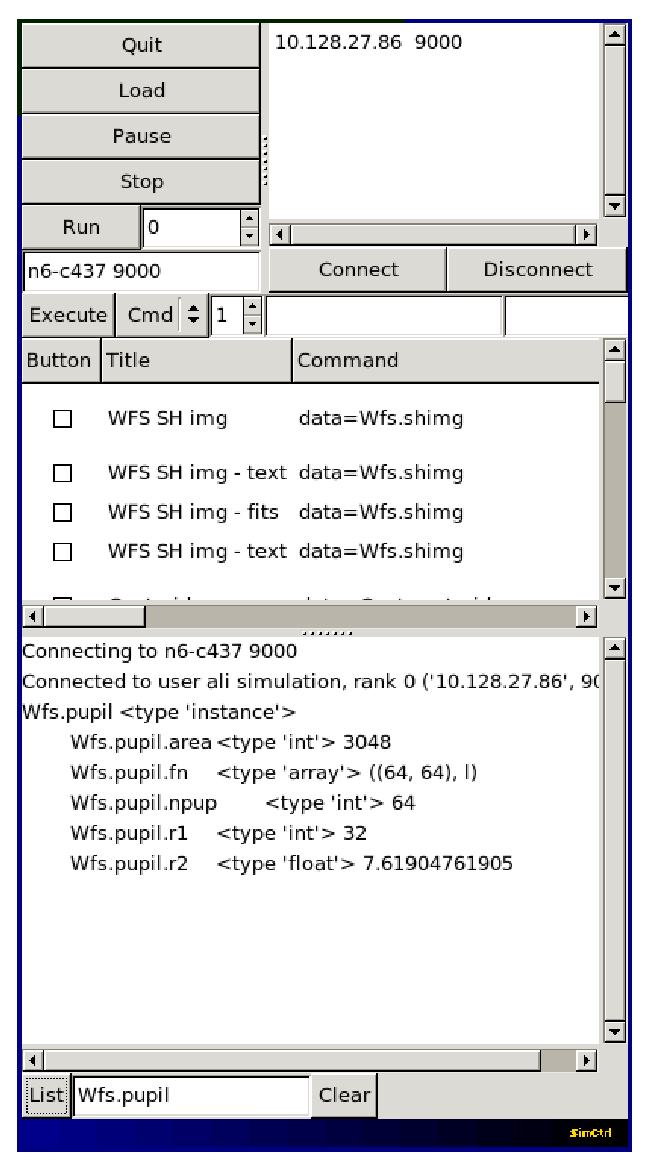
\includegraphics{pics/simctrlmain.eps}
\caption{A screenshot of the simulation control GUI during use}
\label{fig:simctrl}
\end{figure}

\subsection{The main window}
As shown in Fig.~\ref{fig:simctrl}, the simulation control GUI is
divided into several sections, namely a connection list, a button
pannel, an execution panel (including a functionality list), a message
window and a simulation list button bar.


\subsection{The execution panel}
The execution panel consists of an Execute button and an associated
selection box and two text boxes.  It also includes the functionality
list.

In the functionality list, the current button-click operations that
can be used (defined in an XML file) are displayed.  This list has
several columns, but for a casual user, only the first two ({\bf
  Button} and {\bf Title}) are important.  A description of these
columns is provided here:
\begin{description}
\item[Button] Contains a button which can be clicked or toggled to
  carry out the function given in the other columns on the simulation.
\item[Title] A textual description of what the button does, or what it
  returns.
\item[Command] The command which will be executed by an \texttt{exec}
  command in the simulation.
\item[Return] The name of the variable to be returned.
\item[Type] The operation to be carried out on the data, i.e.\ whether
  to plot, save or display the data.
\item[Preprocess] Code that can be used to preprocess the data.
\item[Post] Code that can be used to post-process the data, for
  example to save Gist plots.  This code has access the the global
  dictionary.
\item[Dimensions] The dimensions that should be used when plotting the
  data (i.e.\ a graph or a 2D plot).
\item[Xaxis] The values used for the x axis in the case of a 1D plot.
\item[When] The type of execution required, determining whether the
  command should be executed immediately, at the end of the current
  iteration, or at the end of every iteration.
\item[Options] A python dictionary of further options that can be used
  when handling the data, for example, the palette to use when
  displaying data plots.
\end{description}
When a button is clicked, the relevant command will be sent to all
connections selected in the connection list window (if none are
selected, the command is sent to all connections).  

The functionality list is selected by clicking the {\bf Load} button,
and the user must then select an XML file.

\subsubsection{Functionality list file format}
The functionality list files must be in XML format, and have the
following specification.

The base XML tag should be $<$simdata$>$.  Within this tag, $<$plot$>$ tags
should be placed.  Each of these plot tags can have the following
attributes:

\begin{description}
\item[title] (Optional) A title that is meaningful for a user, e.g. Shack
  Hartmann Images.
\item[cmd] The command to be executed by the simulation.
\item[ret] The object to be returned to the GUI.
\item[type] (Optional) What to do with the data.  Could be e.g. gist, pylab,
  text, save, None.
\item[gisttype] (Optional) Equal to one to display data with Gist.
\item[pylabtype] (Optional) Equal to one to display data with pylab.
\item[texttype] (Optional) Equal to one to display data as text.
\item[savetype] (Optional) Equal to one to save data.
\item[when] (Optional) When to execute the command, one of ``now'', ``cmd'' or
  ``rptN'' where N is the frequency at which it should be carried out
  (or every iteration if not present).
\item[preprocess] (Optional) This can be either an attribute, or the
  text between the opening and closing $<$plot$>$ tags.  This is python
  code which gets executed (using the exec command) on the data, and
  so the data can be handled in an arbitrary way.  This can be used
  for rescaling data etc.\ before plotting.  Within this code,
  assignment to ``button'' is allowed, which will determine the state
  of the button in the functionality list (i.e.\ toggled or not).
\item[post] (Optional) This can be either an attribute, or specified
  withing $<$post$>$ tags inside the $<$plot$>$ tag, and is python
  code which gets executed (using the exec command in the global name
  space) and can be used for post processing, for example to save Gist
  plots.  
\item[dim] (Optional) The dimensions of the data (1 or 2), used when
  plotting the data.
\item[xaxis] (Optional) Can be used if dim=``1'' to specify the x
  axis.  The string is eval'd so for example, Numeric.arange(100)
  would work.  If xaxis is not specified, then if data is a 1D array,
  an xaxis is created the length of data.shape[0].  If data is 2D
  array, xaxis is taken as data[0] and the values (possibly multiple
  lines) are data[1:]
\item[Further options] Further options can be used, depending on the
  type of the object.
  \begin{description}
    \item[gist] palette to specify the palette, e.g.\ gray.gp, window
    to specify the Gist window number, e.g.\ 1, 2 etc.
    \item[text] wintype to specify where to display the text, one of
    ``ownwindow'' or ``mainwindow'', and textreplace (1 or 0) to
    determine whether to append or replace text when new data arrives.
    \item[save] filetype (fits, cvs or text), filename and filereplace
    (1 or 0) to specify whether to overwrite or append when new data
    arrives.
    \item[pylab] No arguments yet.
    \item[None] No arguments.
  \end{description}
\end{description}

As a short example, the XML file could read as follows:
\begin{verbatim}
<simdata>
<plot title='SHWFS image' cmd='data=wfs.shimg' ret='data' type='gist' palette='gray.gp'/>
</simdata>
\end{verbatim}

\subsubsection{Advanced execution}
An advanced user can insert text to be executed in the first text box
next to the execute button, and optionally, add a return value in the
second text box.  By selecting one of ``cmd'', ``rpt'', ``now'' or
``del'', the user can define when the command should be executed, and
(if ``rpt'' is selected) the frequency at which it should occur using
the spin button.  Once the Execute button is pressed, this code will
be executed by the simulation, and any requested results returned.
Currently, these results will be displayed in the message window, but
future versions of the simctrl.py program may allow the user to
operate on this data.

\subsection{The message window}
The message window typically contains warning message if a mistake has
been made, messages from the simulation, any unexpected data from the
simulation, and other information relevent for the user.

\subsection{The connection list}
The connection list displays the currently connected simulation
processes, giving the host name and port number.  The user can
disconnect from one or more simulation processes by clicking the
disconnect button (if no process is selected, all will be
disconnected).  Additionally, by adding a host name and port number in
the text box to the left of the connect button and pressing the
connect button, a new simulation process can be connected to.

\subsection{The button panel}
The button panel contains buttons to control the simulation execution
and select a file for the functionality list, as well as close the
GUI.  These buttons are as follows:
\begin{description}
\item[Quit] Quit the GUI (disconnecting from any open simulations).
\item[Load] Allows the user to select a new XML file from which the
  functionality list will be created.
\item[From sim] Gets the simulation to generate the XML file from
  which the functionality list is created, and then passes this to the GUI.
\item[Pause] Pause selected simulation processes at the end of the current
  iteration (if no processes are selected, pause all).
\item[Stop] End the selected simulation processes at the end of the
  current iteration (if no processes are selected, stop all).
  Currently, now warning message is displayed when this button is
  clicked, though future versions may implement this feature.
\item[Run] Run the selected simulation processes for the number of
  iterations specified in the box to the right of the Run button.  If
  this number is zero, will run until the simulation ends, or is
  paused.  If no simulation processes are selected, all processes will
  be run.
\end{description}

\subsection{The simulation list button bar}
The simulation list button bar consists of a {\bf List} button, which
when pressed will print all the simulation objects in the message
window.  If there is text in the text box to the right of the {\bf
  List} button, this text will be used to select which objects to
list.  Currently, the exact object name must be inserted, though there
are plans to allow a regular expression pattern match instead.  
The {\bf Clear} button to the right of this can be used to clear the
message window.  

Fig.~\ref{fig:simctrl} shows an example of this List functionality in
the message window, when the {\bf List} button has just been clicked.

\section{The simulation analyser}
The simulation analyser (analyse.py) can be imported into an existing
interactive Python session, and used to connect to one or more
simulation processes.  Once an analyse object has been initialised,
new connections can be opened using the {\bf openConnection} method
(and closed using the {\bf closeConnection} method).  

The simulation can be paused, run or stopped using the {\bf pause},
{\bf run} and {\bf stop} methods, specifying the connections to which
this applies (if no connections are selected, the command will be
applied to all open connections).

The {\bf getObjects} method will return a text
string containing all selected objects in the simulation, functioning
in a similar way to the {\bf List} button in the simctrl.py GUI.  

The {\bf execute} method can be used to execute arbitrary code within
the simulation, and callbacks can be added to handle any data returned
using the {\bf addCallback} method.  The {\bf process} method can be
used to process any callbacks for which data has arrived.  

The {\bf read} methods (several variants) can be used to read the open
sockets (or a list of sockets provided by the user) and will return a
list of lists for each data item ready for reading, with each of these
lists containing the socket from which data was received, and the
data.  The user can then act on the data as appropriate.  For
convenience, a {\bf getData} method is defined, which takes no
arguements, and returns a list of any available data, without any
information about the socket or tag corresponding to this data.  This
is best used when only one socket is open, and you are expecting only
one piece of data to be returned.

\section{Conclusion}
The simulation control methods (textual and graphical) have been
described, and you should now be able to use them (possibly in
conjunction with the API reference for the textual case).

\section{Work to do}
There are a number of things that could do with improvement in the
simctrl GUI.

DONE: A feature which is desirable is to be able to get a command history of
things entered in the ``command to be sent'' entry box, or even to
have a mini python interpreter embedded here.  Additionally, data
returned here should have the option of plotting, rather than
printing.

Another thing that is desirable is to have paned tick boxes, one for
each connection.  Or something similar, i.e.\ a way to determine if
you have several connections, which ones have which boxes ticked.
Maybe it needs a column of tick boxes for each connection, plus a
global column.  Then you can either click links individually, and see
them ticked, or set/unset them all.


That should keep someone busy for a couple of weeks anyway!
\bibliography{references}
\printindex
\end{document}
